\documentclass[12pt]{article}

\usepackage{url}
\usepackage[utf8]{inputenc}
\usepackage[english,russian]{babel}
\usepackage{tocvsec2}

\usepackage[dvips]{graphicx}
\graphicspath{{images/}}

\usepackage{tikz}
\usepackage{listings}

\renewcommand{\rmdefault}{ftm}
\usepackage[T2A]{fontenc}
\usepackage{setspace}
\setstretch{1.5}

\usepackage{geometry}
\geometry{top=2cm}
\geometry{bottom=2cm}
\geometry{left=3cm}
\geometry{right=1.5cm}

\renewcommand\contentsname{Содержание}
\setcounter{tocdepth}{2}

\renewcommand{\baselinestretch}{1.5}

\begin{document}
	
	{\thispagestyle{empty}
		\begin{center}
			\scriptsize Министерство образования и науки Российской Федерации\\
			\scriptsize Федеральное государственное автономное образовательное учреждение высшего образования\\
			\normalsize\bf <<Уральский федеральный университет\\
			\normalsize\bf имени первого Президента России Б.Н. Ельцина>>
		\end{center}
		
		\begin{center}
			\normalsize\bf Институт естественных наук и математики\\
			\normalsize\bf Департамент математики, механики и компьютерных наук\\
		\end{center}
		
		\vspace{3cm}
		
		\begin{center}
			\LARGE\bf Исследование потокобезопасных неблокирующих структур данных
		\end{center}
		
		\vspace{2.5cm}
		
		\hspace{-1cm}
		\begin{minipage}{80mm}
			\noindent
			\vspace{-2.3cm}
			\begin{flushleft}
				\begin{spacing}{1.0}
				\large <<Допущен к защите>>\\
				\underline{\hspace{6cm}}\\
				\large Директор департамента\\
				\large к.ф.-м.н., доцент\\
				\large Асанов~М.~О.
				\underline{\hspace{6cm}}\\
				<<\underline{\hspace{0.7cm}}>>\underline{\hspace{3cm}}2017 г.
				\end{spacing}
			\end{flushleft}
		\end{minipage}
		\begin{minipage}{90mm}
			\begin{flushleft}
				\begin{spacing}{1.0}
				\large Квалификационная работа на соискание степени бакалавра наук по направлению\\
				\large <<Фундаментальная информатика и информационные технологии>>\\
				\large студента группы ФТ-401 (МЕН-430802) Сваловой~А.~А.\\
				\large Научный руководитель:\\
				\large Ассистент департамента к.ф.-м.н.\\
				\large Плинер~Ю.~А.
				\end{spacing}
			\end{flushleft}
		\end{minipage}
		
		\vfill
		
		\begin{center}
			Екатеринбург\\
			2017 год
		\end{center}
	}

	\newpage
	
	{\pagestyle{plain}
		\tableofcontents
	}

	\newpage
	
	{\pagestyle{plain}
		
		\section{Введение}
			\par\large С ростом прогресса многие электронные устройства становятся многоядерными, появляются многопроцессорные устройства. Поэтому задача программиста, как человека, который пытается максимально хорошо использовать предоставленные ресурсы, - писать программы, способные масштабироваться и параллелиться. Поэтому сейчас все чаще и чаще пишут многопоточные программы и используют многопоточные структуры данных. Такие программы могут выполнять сразу несколько инструкций на каждом процессоре или ядре, однако такой код обладает рядом проблем, связанных с доступом к общим ресурсам разными потоками или процессами.
			\par Если два или более потока захотят изменить один и тот же участок памяти, то они попытаются сделать это единовременно. После выполнения операции неизвестно, как будет выглядеть этот участок памяти, так как порядок выполнения инструкций разных потоков неопределен. Возникает вопрос: как в таком случае контролировать доступ к этому ресурсу? Хочется чтобы в каждый момент времени, способом, очевидным для разработчика, ресурсом владел только один поток, а все остальные каким-то образом ждали своей очереди. Такое поведение можно осуществить несколькими способами. 
			\par Самый простой из них - блокировка. Каждый раз, когда поток хочет сделать что-то с ресурсом, он проверяет, нет ли блокировки на этот ресурс. Если есть, поток ждет, пока блокировка не освободится, если нет, то он пытается первым захватить блокировку. В случае успешного захвата он осуществляет все операции с ресурсом и освобождает блокировку. В это время все остальные потоки ждут этот и ничего не делают. 
			\par Такой механизм синхронизации очень прост в понимании и реализации, учитывая существование встроенных блокировок в большинство современных ОС. Также этот способ, очевидно, позволяет только одному потоку единовременно получить доступ к ресурсу. Однако, в данном способе существует и масса проблем, которые сводят на нет все преимущества. Во-первых, при большом количестве потоков, желающих получить доступ к ресурсу, возникает <<узкое горлышко>>, т. е. место в программе, которое тормозит выполнение программы в целом. Во-вторых, при существовании больших участков программы с блокировкой теряется весь смысл многопоточности. В эти участки все равно может заходить только один поток, как и в однопоточном программировании. В-третьих, существуют некоторые особенности операционной системы: переключение потоков - дорогая операция. При долгом ожидании освобождения ресурса происходит очень большое количество переключений, следовательно, большое количество времени тратится на бесполезные операции. В-четвертых, возможны ситуации, когда один поток захватил первый ресурс и ждет освобождение второго ресурса, в то время как второй поток захватил второй ресурс и ждет освобождения первого. Такая ситуация называется взаимная блокировка (deadlock). Программа в таком случае останавливает свое выполнение совсем и не может без каких-либо вмешательств извне разрешить эту ситуацию.
			\par Эти проблемы привели исследователей к созданию других способов синхронизации. Один из них - неблокирующая синхронизация. Это способ, при котором каждый поток пытается применить низкоуровневые атомарные аппаратные примитивы, а не использовать блокировки. Таким образом в каждый момент времени выполняется только одна операция, только одного потока. Все остальные операции в других потоках либо завершаются ошибкой, либо выполняются сразу следом за предыдущей. Такие алгоритмы обеспечивают общее продвижение программы в целом: даже если какой-то поток не смог выполнить операцию или завершился с ошибкой - значит, что какой-то другой поток успешно выполнил свою операцию. Не существует случаев, когда все потоки одновременно простаивают, и как частный случай этого, невозможно существование взаимных блокировок. 
			\par Однако, несмотря на все преимущества, данная область является до сих пор развивающейся. Нельзя просто взять и написать неблокирующую реализацию алгоритма, основанного на блокировках. В некоторых случаях это оказывается легко, в некоторых до сих пор не придумано неблокирующих аналогов. Причина: каждый раз нужно творчество, чтобы свести все операции над разделяемым ресурсом к последовательности независимых атомарных операций, т. е. не существует универсального способа написания неблокирующей реализаци. Однако сложность реализации и изобретения алгоритма часто стоит усилий. Пусть этот класс алгоритмов совсем не о скорости работы, а о гарантии продвижения системы в целом, но в итоге большинство неблокирующих алгоритмов имеют в среднем ожидаемую сложность меньше, чем блокирующие аналоги. Но это только в теории. На практике скорость работы зависит от конкретной реализации, области применения, часто встречающихся запросов и т. д.
			\par Цель данной работы: реализовать основные структуры данных, реализующие интерфейс ISet и на практике выявить являются ли неблокирующие алгоритмы эффективней блокирующих, какие алгоритмы вообще реально применимы, и выяснить, как адаптировать алгоритмы, разработанные под языки программирования с неуправляемой памятью, к языкам с управляемой памятью.
			\par В работе представлены структуры данных, реализующие интерфейс ISet. Данный интерфейс включает в себя добавление элемента в множество, удаление элемента, а также поиск и перечисление всех элементов в множестве. Этих сценариев достаточно, чтоб понять, как ведут себя различные реализации на практике. Для сравнения были выбраны следующие реализации: сортирующийся лист, хэш-таблица, скип-лист и дерево поиска. Также взяты готовые реализации всех этих структур из библиотеки языка C\#, чтобы сравнить неблокирующие реализации с блокирующими. В приложении приведены различные результаты сравнений всех этих структур и вариации использования их в реальной жизни. Все алгоритмы адаптированы под язык C\# и собраны в один общий модуль с внешним интерфейсом ISet.
		
		\newpage
		
		\section{Глава 1. Основные определения}
			\subsection{Атомарная операция (Обсудить, нужны ли картинки и сколько)}
				\par Все неблокирующие алгоритмы можно разделить на три типа: Waitfree, Lockfree, Obstruction-free\cite{WaitFree}.
				\par В первом типе каждый поток совершает каждую операцию за конечное число шагов, независимо от влияния других потоков. это самое сильное требование из-за чего редко реализуемое. Такие алгоритмы обычно реализуют атомарный инкремент или атомарную замену ссылок.
				\par Во втором типе система в целом двигается вперед, даже если какой-то поток стоит на месте. Если какой-то поток не смог выполнить операцию, значит, что какой-то другой поток смог выполнить свою операцию, следовательно, в целом система продвинулась. Эти алгоритмы обычно реализуют атомарное сравнение и замену.
				\par В третьем типе каждый может выполнить каждую операцию за конечное количество шагов, если ничего ему не помешает. В данном случае может случиться ситуация, когда ни один из потоков не двигается вперед, однако ни один заблокированный поток не может мешать работе всех остальных потоков, следовательно, это все равно более сильная гарантия, чем блокирущие алгоритмы.
				\par Каждая из этих реализаций использует абстракцию <<атомарная операция>> - это операция, которая либо не выполняется совсем, либо выполняется как единое целое. В данной работе используется атомарная операция Compare~And~Swap~(CAS). Эта операция сравнивает две ссылки и, если они равны, меняет первую на данную третью. Эта операция предоставляется большинством операционных систем и уже встроена в язык C\#.
			\subsection{Atomic markable reference}
				\par Алгоритмы с неблокирующей синхронизацией оказываются в разы сложнее обычных алгоритмов. Зачастую, они зависят от конкретной реализации или конкретного языка программирования. Иногда они полагаются на сборщика мусора (абстракцию в языках программирования с управляемой памятью) или, наоборот, его отсутствие. Кроме того, доказать корректность таких алгоритмов бывает очень сложно. Поэтому со временем стали придумывать не только алгоритмы с неблокирующей синхронизацией, но и комбинации, где особо часто используемые операции производятся без блокировок, а некоторые операции производятся с блокировками, но на маленькие участки памяти. Такие алгоритмы оказываются проще в понимании и доказательстве, но не проигрывают в эффективности и применимости.  
				\par Один из способов такой локальной блокировки - это добавление особого маркера в ссылку на объект. Так, если один поток смог атомарно изменить ссылку на некий объект, пометив ее этим маркером, все остальные потоки понимают, что данный объект используется в какой-то операции и его нельзя изменять. 
				\par В языках с неуправляемой памятью такой способ легко осуществим благодаря выравниванию указателей на объект. При выделении памяти компилятор, обычно, выравнивает длину указателя на максимально большой тип данных. Поэтому в указателе остаются реально неиспользуемые биты, которые можно как раз и использовать в качестве маркера.
				\par В языках с управляемой памятью разработчик не имеет доступа к ссылке, поэтому стоит придумывать способы сымитировать эту ссылку с помощью объектов. В данной работе реализован примитив маркируемой ссылки (Atomic Markable Reference), который состоит из ссылки на объект и состояния этой ссылки. В данном случае состояние как раз отвечает за неиспользуемые биты указателя. Изменяя этот примитив, можно сымитировать изменение указателя, что позволяет также использовать алгоритмы с локальными блокировками.			
			\subsection{SpinWait}
				\par (обсудить, действительно ли нужно писать об этом. я разобралась в нем)
		
		\newpage
		
		\section{Глава 2. Реализации алгоритмов}
			\par В данной главе будут приведены краткие описания неблокирующих алгоритмов, проблемы, которые они решают и сложности реализации. Полное описание алгоритмов можно найти в списке литературы \cite{LinkedList}, \cite{ListSkipList}, \cite{ListAndSkipList}, \cite{HashTable}, \cite{artOfMultiprocessor}. Стандартные реализации однопоточных алгоритмов общедоступны, поэтому не будут описаны в данной работе. Познакомиться с ними можно, например, в книге <<Структуры данных и алгоритмы>> \cite{dataStructures}.
			\subsection{Односвязный список}
				\par Пусть односвязный список состоит из элементов, в каждом из которых есть значение этого элемента и ссылка на следующий элемент. Поиск элемента не будет рассмотрен, так как он совпадает с поиском в обычном сортирующимся списке.
				\begin{figure}[h]
				\begin{lstlisting}
public class LinkedListNode<TElement>
{
	TElement Element;
	LinkedListNode<TElement> Next;
}
				\end{lstlisting}
				\caption{Вершина списка}
				\end{figure})
				\par Если реализовать добавление как в однопоточном варианте, то возможна проблема при одновременном добавлении двух последовательных элементов. Пусть, есть список с элементами \textbf{1}-\textbf{2}-\textbf{5} (Рис~2a). Поток \textbf{А} хочет вставить элемент \textbf{3}, поток \textbf{Б} - элемент \textbf{4}. Поток А понимает, что ему нужно вставить элемент между \textbf{2} и \textbf{5}. Он запоминает ссылку на предыдущий и следующий элементы и в этот момент операционная система передает управление потоку \textbf{Б} (Рис~2b). Поток \textbf{Б} также находит место для вставки и тоже запоминает \textbf{2}, как предыдущий элемент, \textbf{5}, как следующий (Рис~2c). После этого он переписывает ссылку <<Следующий>> у элемента \textbf{2} на новосозданный элемент \textbf{4}, а у элемента \textbf{4} на \textbf{5} (Рис~2d). Управление возвращается к потоку \textbf{А}. Он перезаписывает ссылку <<Next>> предыдущего элемента \textbf{(2)} на новосозданный элемент \textbf{3}, а ссылку элемента \textbf{3} на следующий элемент \textbf{(5)} (Рис~2e). В результате элемент \textbf{4} <<потеряется>>, т. е. не будет ни одной ссылки, указывающей на него.
				\par
				\begin{figure}[h]
					\begin{minipage}[h]{0.45\linewidth}
						\center{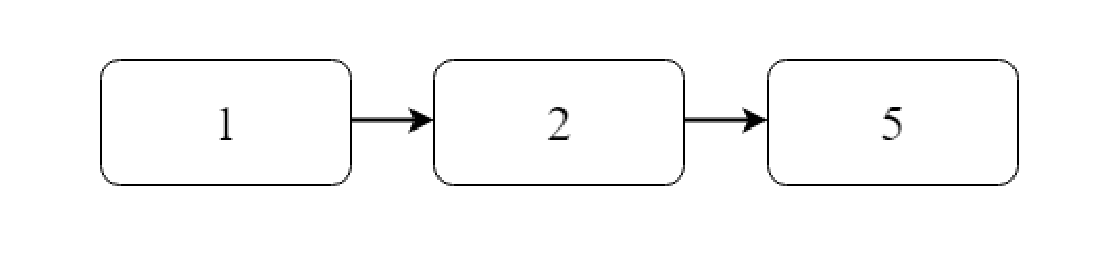
\includegraphics[width=1\linewidth]{1}} a) \\
					\end{minipage}
					\hfill
					\begin{minipage}[h]{0.45\linewidth}
						\center{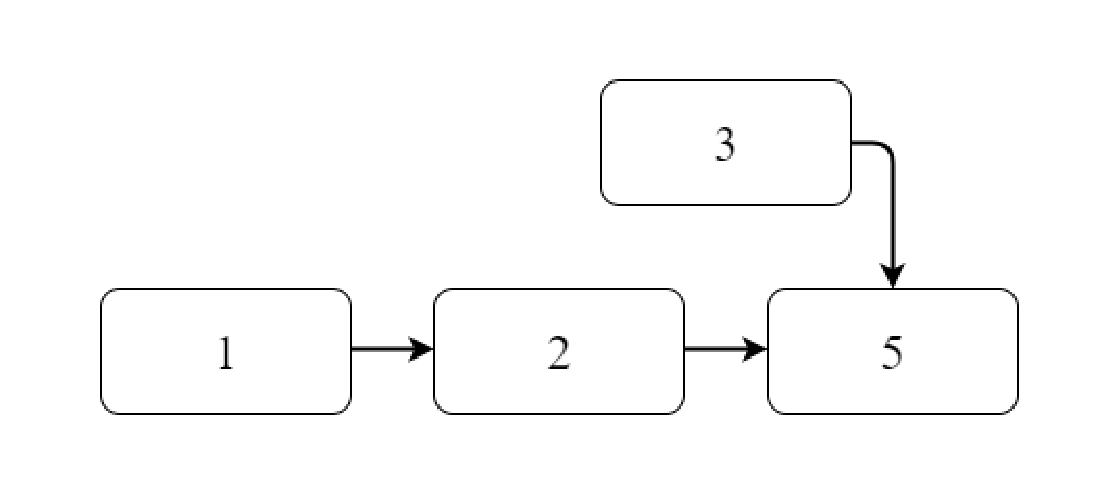
\includegraphics[width=1\linewidth]{2}} \\b)
					\end{minipage}
					\vfill
					\begin{minipage}[h]{0.45\linewidth}
						\center{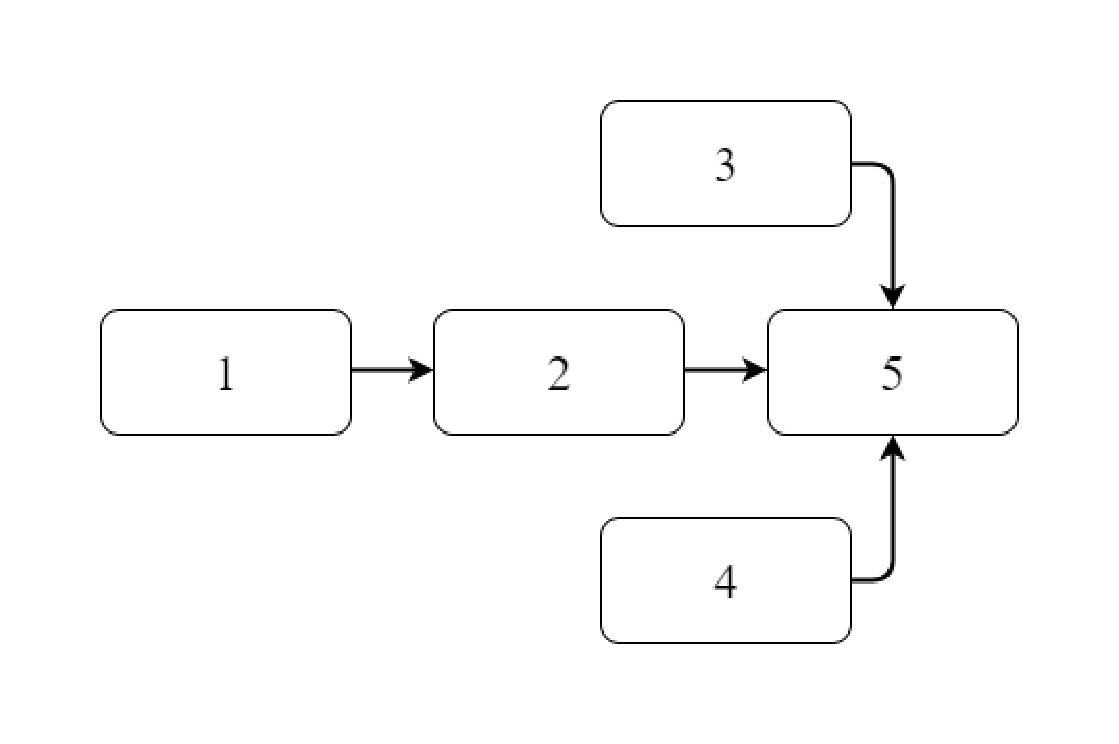
\includegraphics[width=1\linewidth]{3}} c) \\
					\end{minipage}
					\hfill
					\begin{minipage}[h]{0.45\linewidth}
						\center{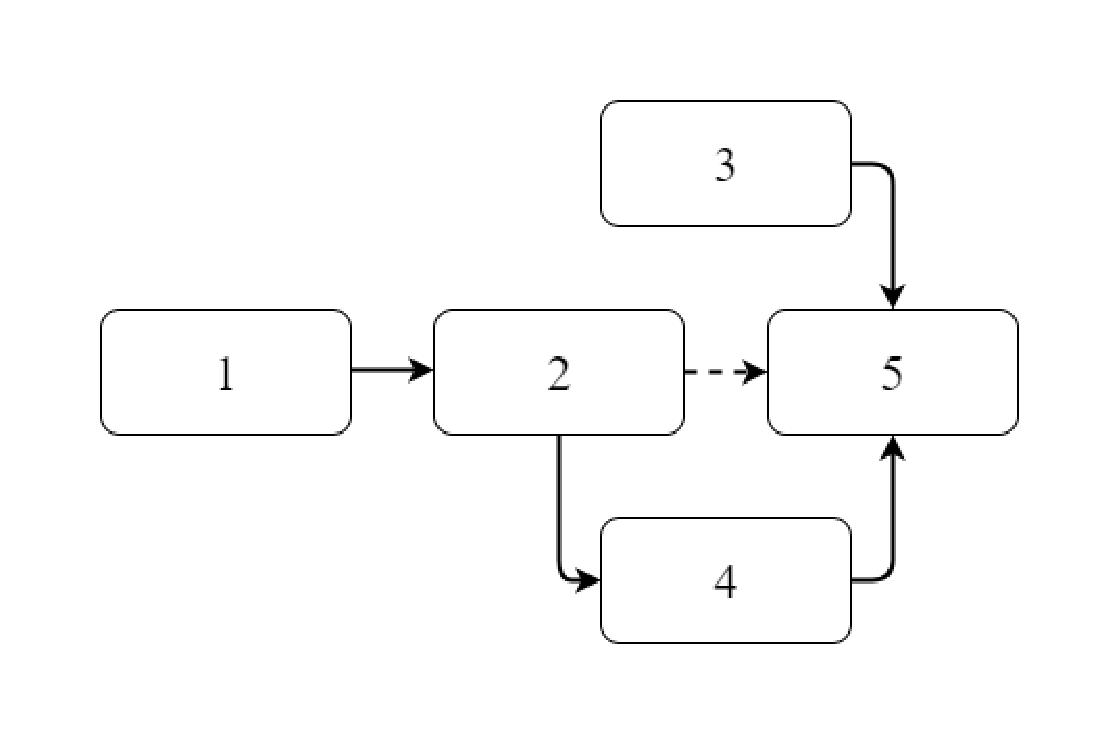
\includegraphics[width=1\linewidth]{4}} d) \\
					\end{minipage}
					\begin{minipage}[h]{0.45\linewidth}
						\center{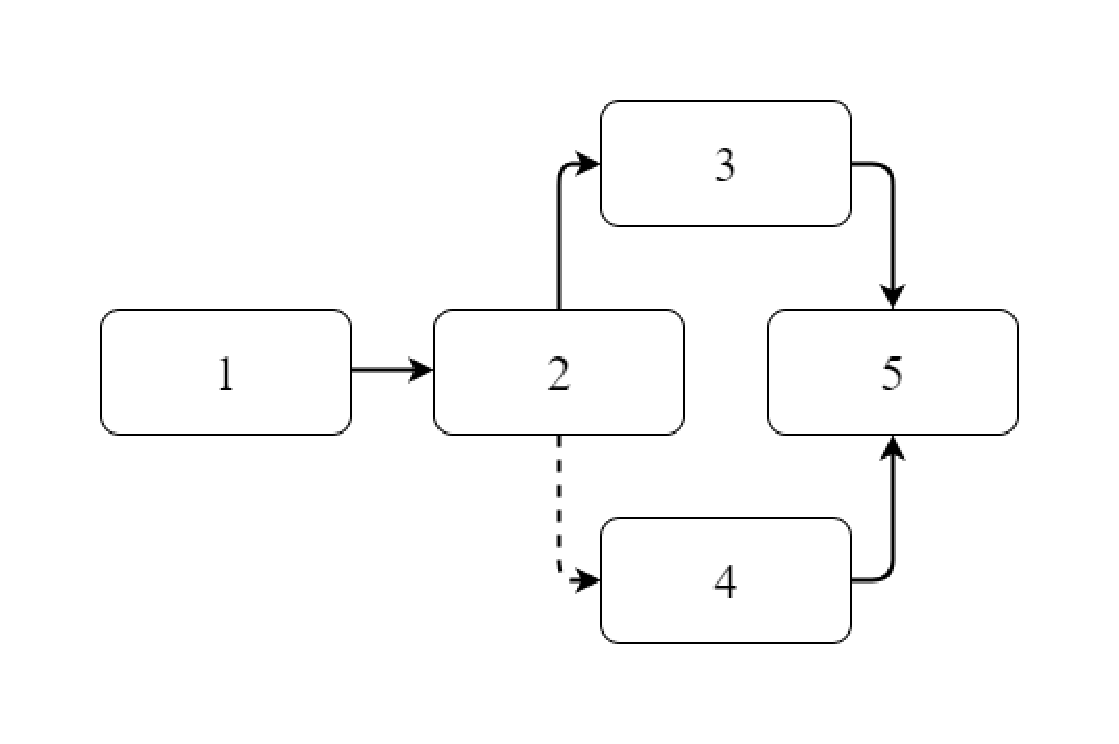
\includegraphics[width=1\linewidth]{5}} e) \\
					\end{minipage}
					\caption{Одновременное добавление в 2 потоках: a) начальное состояние, b) А поставил ссылку на 5, c) Б поставил ссылку на 5, d) А сменил ссылку <<Next>> у 2, e) Б сменил ссылку <<Next>> у 2.}
					\label{ris}
				\end{figure}
				\par Реализация неблокирующего доступа использует типичный прием для неблокирующих алгоритмов - вечный цикл с операцией CAS. На каждом шаге цикла алгоритм пытается найти два элемента \textbf{а} и \textbf{б}, между которыми должен быть вставлен новый, и атомарно перезаписать ссылку <<Next>> с предыдущего элемента \textbf{(а)} на новый, при этом сравнивая, является ли эта ссылка до сих пор ссылкой на следующий \textbf{(б)}. Алгоритм выходит из цикла, когда попытка замены ссылки происходит успешно. Такая реализация полностью решает вышеописанную проблему. При попытке перезаписать ссылку элемента \textbf{2} с \textbf{5} на \textbf{3}  (Рис~2e), CAS не проходит, потому что ссылка уже не на \textbf{5}, а на \textbf{4}. Алгоритм заново находит соседние элементы, и следующий уже не \textbf{5}, а \textbf{4}. На этом шаге цикла CAS уже выполняется успешно. Оба элемента вставлены правильно.
				\par Еще одна проблема может возникнуть при одновременным удалении и вставке двух последовательных элементов. Пусть есть список \textbf{1}-\textbf{2}-\textbf{4} (Рис~3a). Поток \textbf{А} хочет добавить элемент \textbf{3}, поток \textbf{Б} удалить элемент \textbf{2}. Поток \textbf{Б} запоминает, что предыдущий элемент \textbf{1}, следующий \textbf{4}. Управление передается потоку \textbf{А}. Поток \textbf{А} вставляет элемент \textbf{3}, как это было описано ранее (Рис~3b). Управление возвращается к потоку \textbf{Б}. Он атомарно заменяет ссылку <<Next>> у элемента \textbf{1} на элемент \textbf{4} (Рис~3c). В итоге элемент \textbf{3} <<потерялся>>.
				\begin{figure}[h]
					\begin{minipage}[h]{0.45\linewidth}
						\center{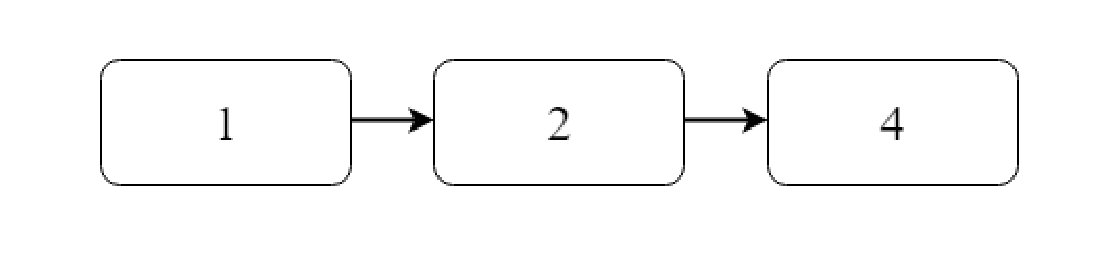
\includegraphics[width=1\linewidth]{6}} a) \\
					\end{minipage}
					\hfill
					\begin{minipage}[h]{0.45\linewidth}
						\center{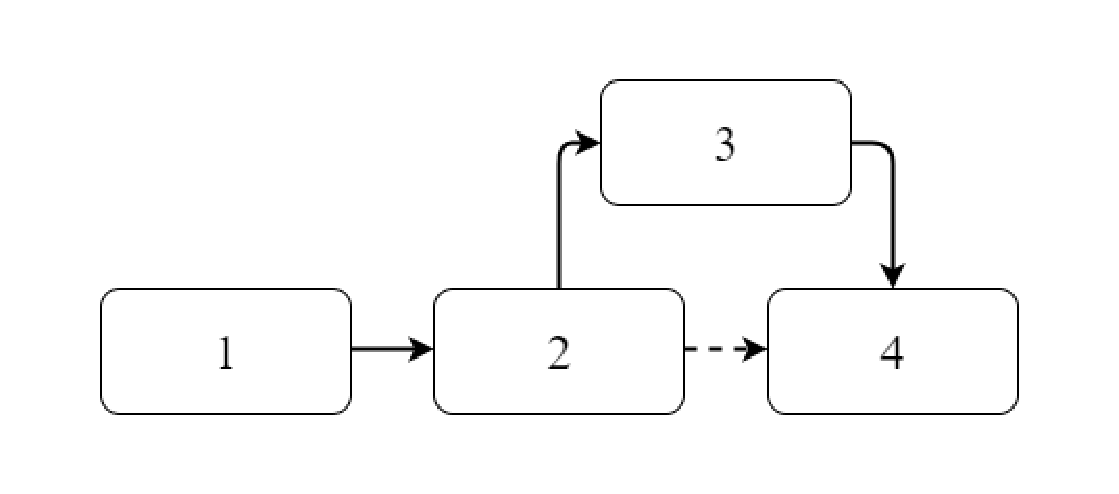
\includegraphics[width=1\linewidth]{7}} \\b)
					\end{minipage}
					\vfill
					\begin{minipage}[h]{0.45\linewidth}
						\center{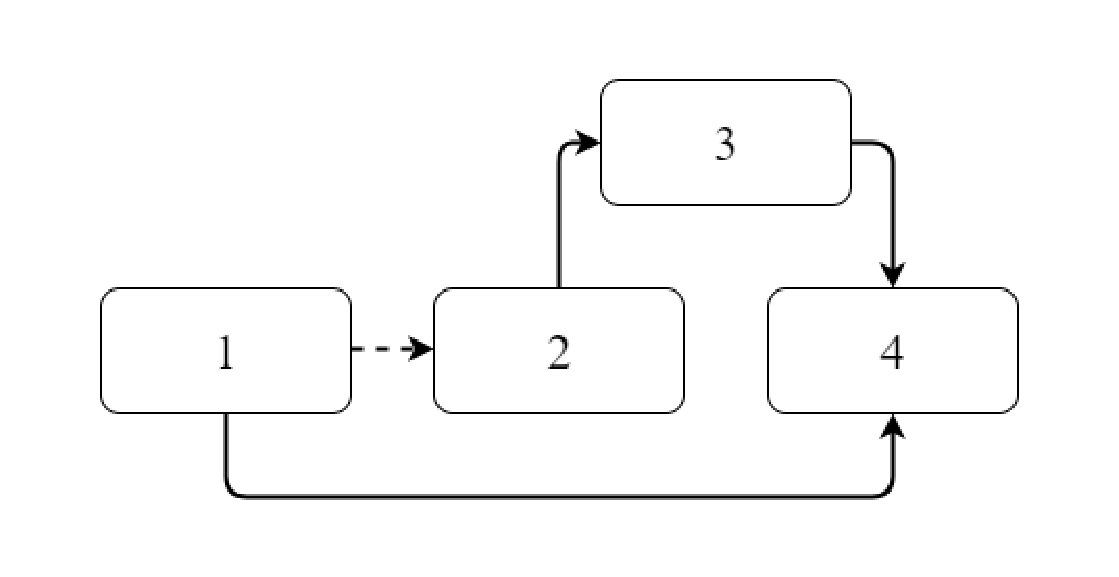
\includegraphics[width=1\linewidth]{8}} c) \\
					\end{minipage}
					\caption{Одновременное добавление и удаление в 2 потоках: a) начальное состояние, b) А поставил ссылку на 4, c) Б сменил ссылку с 2 на 4.}
				\end{figure}
				\par Для устранения этой проблемы можно ввести дополнительный флаг в ссылку на объект (Рис~4).
				\begin{figure}[h]
					\begin{lstlisting}
public class LinkedListNode<TElement>
{
	TElement Element;
	AtomicMarkableReference<LinkedListNode<TElement>, Flag> Next;
}
					\end{lstlisting}
					\caption{AtomicMarkableReference - структура, описанная в предыдущей главе, Flag может быть никаким или помеченным}
				\end{figure}
				\par Теперь объект удаляется в два шага: 
				\begin{itemize}
					\item пометить как удаленный, но не удалить
					\item физически удалить. 
				\end{itemize}
				Можно заметить, что при помечивании ссылки на удаленный элемент, ситуация, изображенная на рисунке 2, существенно не изменится. Однако, при помечивании ссылки <<Next>> у удаляемого объекта, можно избежать петерь элементов. Теперь при вставке тройки из предыдущего примера ссылка <<Next>> у \textbf{2} уже будет помеченной. Это будет сообщать о том, что элемент в данный момент удаляется, а значит, манипулировать этой ссылкой пока что нельзя, надо заново перейти на новый виток в цикле и заново определить соседей. В итоге проблемы, описанной ранее при одновременной вставке и удалении не случится.
			\subsection{Улучшенный односвязный список}
				\par Вышеописанная реализация односвязного списка является неблокирующей, что, возможно, может ускорить работу программы, однако у нее до сих пор существует недостаток: если операции удаления происходят достаточно часто, то операции вставки будут также часто заканчиваться не успехом, из-за чего они каждый раз начинать сначала. В результате в худшем случае может получиться, что программа каждый раз заново пробегает весь список.
				\par Чтобы устранить эту проблему можно ввести еще две дополнительных абстракции. В ссылку <<Next>> добавить еще один флаг, который будет свидетельствовать, что следующий элемент в данный момент на стадии удаления. В сам элемент нужно добавить поле <<Backlink>>, который будет указывать на предыдущий элемент, который еще не участвует в удалении (Рис~5). 
				\begin{figure}[h]
					\begin{lstlisting}
public class LinkedListNode<TElement>
{
	TElement Element;
	LinkedListNode<TElement> Backlink;
	AtomicMarkableReference<LinkedListNode<TElement>, Flag> Next;
}
					\end{lstlisting}
					\caption{AtomicMarkableReference - структура, описанная в предыдущей главе, Flag может быть никаким, или помеченным на удаление, или помеченным на невозможность удаления}
				\end{figure}
				Теперь операция удаления будет проходить не в два, а в три этапа. Между двумя этапами из предыдущего алгоритма появится новый этап. Теперь после помечивания удаляемой вершины на удаление (Рис~6a) алгоритм добавляет в ссылку <<Next>> у предыдущей вершины новый флаг, который будет обозначать, что в данный момент вершина участвует в удалении, и ее саму удалять нельзя. У удаляемой вершины алгоритм устанавливает ссылку <<Backlink>> на ближайшую предыдущую вершину, которая еще не помечена новым флагом (Рис~6b). Теперь каждый раз, когда вставка не может завершиться успехом, поток будет по ссылкам <<Backlink>> возвращаться не в самое начало, а в первую вершину, следующая за которой еще не удаляется. Это позволяет еще немного ускорить работу программы, так как при каждой неудачной вставке, возможно, больше не нужно проходить лист полностью заново.
				\begin{figure}[h]
					\begin{minipage}[h]{0.45\linewidth}
						\center{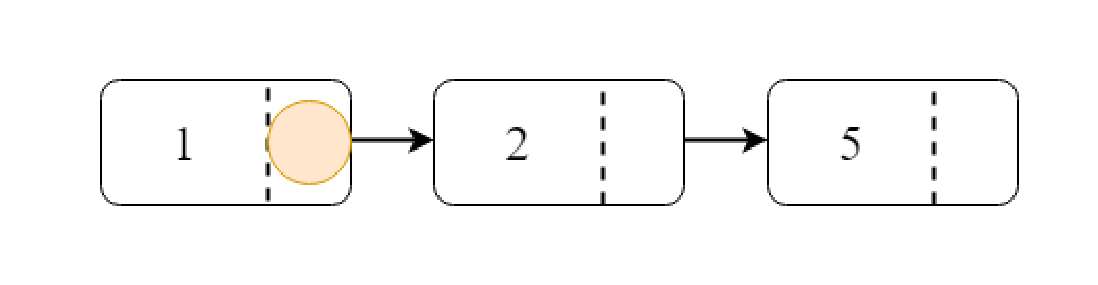
\includegraphics[width=1\linewidth]{9}} a) \\
					\end{minipage}
					\hfill
					\begin{minipage}[h]{0.45\linewidth}
						\center{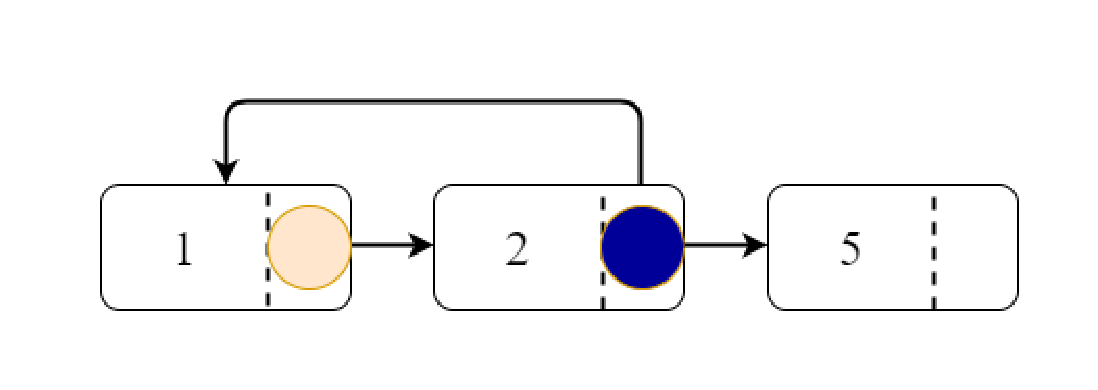
\includegraphics[width=1\linewidth]{10}} \\b)
					\end{minipage}
					\vfill
					\begin{minipage}[h]{0.45\linewidth}
						\center{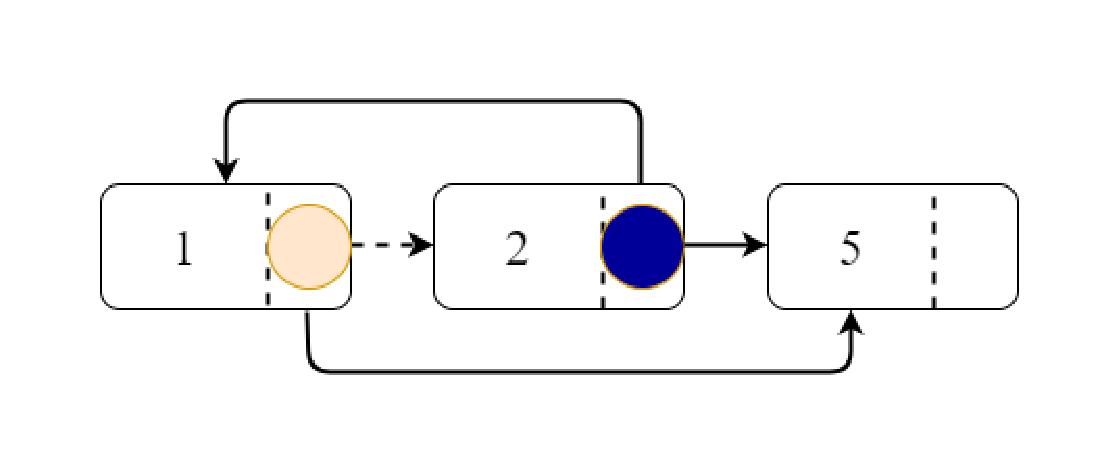
\includegraphics[width=1\linewidth]{11}} c) \\
					\end{minipage}
					\caption{Удаление в 3 этапа: a) помечивание на участие в удалении, b) помечивание на удаление, c) реальное удаление.}
				\end{figure}
			\subsection{Список с пропусками}
				\par Список с пропусками в своей структуре содержит несколько самосортирующихся односвязных списков. Поэтому алгоритм неблокирующего списка с пропусками будет использовать все те же идеи, что и неблокирующий односвязный список. Остается разобраться, как применить все те же идеи, но вставляя и удаляя не 1 элемент, а сразу столбец. 
				\par Вставка, как и в однопоточном варианте осуществляется снизу-вверх. Однако, в данном случае на каждом уровне приходится искать заново, иначе можно запомнить элемент, который какой-то другой поток уже удалил.
				\par Удаление тоже происходит, начиная с удаления вершины на самом нижнем уровне. Этого действия достаточно, чтобы весь столбец считался удаленным. При каждом следующем поиске по списку нужно проверять не удалена ли текущая вершина, а удалена ли ее вершина с первого уровня (вершины реально не удаляются из памяти, но на них больше никто не ссылается, поэтому можно считать, что они больше не принадлежат к списку, так как они недостижимы). Если вершина с первого уровня удалена, то нужно удалить и текущую вершину, а также больше не ссылаться на нее и не строить из нее ссылки на новые вершины.
				\par Списки внутри списка с пропусками можно также улучшить с помощью второго алгоритма.
			\subsection{Хэш-таблица}
				\par Хеш-таблица - структура данных, основывающаяся на массиве с произвольным доступом. На данный момент не придумано алгоритма, как можно реализовать строгий параллельный доступ к одной ячейке памяти на запись. Однако блокировать каждый раз весь массив, очевидно, неправильно. В таких случаях используют другой подход.
				\par Весь массив разбивают на кусочки. Чаще всего используют куски одинаковой длины, распределяя их одновременно по массиву. Куски могут пересекаться или не пересекаться. Во время операции модификации высчитывается нужный хэш, находится место в массиве, где этот элемент должен быть изменен, и блокируется только тот кусок, которому принадлежит данный элемент. После модификации блокировка отпускается.
				\par При увеличении количества элементов количество кусков остается неизменным, однако длина каждого из них увеличивается.
				
		\newpage
		
		\section{Глава 3. Тестирование}
				\subsection{Модульное тестирование}
					\par Во время модульного тестирования проверяются максимально изолированные от внешнего мира части системы. Чаще всего такие тесты мелкие и целенаправленные. Такие тесты как раз определяют, изменилась ли функциональность программы или работает ли данная функция в целом.
					\par Тестирование многопоточного приложения всегда трудно. Приходится каждый раз задумываться о том, как будут работать те или иные функциональности вместе. В данной работе использовано два основных подхода. Первый заключается в тщательном тестировании каждого метода в одном потоке. Тестирование многопоточного приложения всегда должно начинаться с проверки функциональности в однопоточном искусственно-созданном окружении. Далее проверяются простые сценарии в нескольких потоках, чтобы проверить, что они вообще корректно взаимодействуют между собой, т. е. делают то, что от них <<ожидают>> в каждом конкретном сценарии.
					\par Второй подход: <<тестирование грубой силой>>. В этом случае запускается большое количество потоков или выполняется большое количество операций одновременно. При увеличении числа операций вероятность ошибки увеличивается, в этом и заключается данный метод. Однако даже это не гарантирует, что программа работает правильно. В некоторых случаях сценарии неправильной работы кода настолько редки, что можно вообще никогда их не получить ошибку в тестировании, но получить в работе с пользователем.
					\par Отсюда плавно вытекает третий подход: тестирование аналитически. Он заключается в тщательном продумывании всех возможных сценариев, проверки каждой строчки кода, попытки смоделировать выполнение программы и найти потенциальные ошибки. Однако большая проблема данного подхода: <<человеческий фактор>>. Иногда такую проверку все же можно сделать формально и наглядно. В данной в ссылках на алгоритмы приведен подробный анализ корректности работы алгоритма, заключающийся просто в разборе всех возможных сценариев.
				\subsection{Тестирование производительности}
					\par Если тестирование работоспособности программы нужна для проверки, что программа работает корректно, то оценка производительности нужна для представления, реализуема ли вообще эта программа в жизни. Проверяется, соответствует ли время работы или количество используемой памяти теоретическим оценкам. Чаще всего такое тестирование проходит в сравнении с эталоном. В данной работе эталоном представлялся дополнительный алгоритм, основанный на блокировании структуры. Ожидается, что на большом количестве потоков, этот алгоритм будет работать в среднем хуже, чем неблокирующий алгоритм.
					\par Для оценки производительности можно использовать различные метрики. В данной работе рассматривалось несколько различных тестовых окружений, в каждом из которых несколько различных структур данных и варианты работы в 1, 2 и 4 потоках. 
					\par Были произведены тесты на 1, 2 и 4 потоках всех вышеописанных структур данных а также их блокирующих аналогов. В качестве тестового окружения был выбран компьютер Intel Core i7-4790 CPU 3.60GHz (Haswell), ProcessorCount=8 Frequency=3507505 Hz, Resolution=285.1029 ns, Timer=TSC. C\# Clr 4.0.30319.42000, 64bit LegacyJIT/clrjit-v4.6.127.1;compatjit-v4.6.1055.0.
					В качестве тестовых сценариев были выбраны такие как: 
					\begin{itemize}
						\item вставка, удаление, поиск по-отдельности
						\item только вставка и поиск в соотношении 9:1
						\item вставка, поиск и удаление в соотношении 2:7:1			
					\end{itemize}
				
				
		\newpage
		
		\section{Заключение}
		
		\newpage
		%\section{Список литературы}
		\addcontentsline{toc}{section}{Список литературы}
			\bibliographystyle{utf8gost705u}
			\bibliography{biblio}  
		
		\newpage
		
		\section{Приложения}
	}
	
\end{document}